% !TeX program = pdflatex
% !TEX encoding = UTF-8 Unicode
% !TEX spellcheck = de_DE
% !BIB program = biber

\documentclass[10pt,a4paper,DIV=12,parskip=half]{scrarticle}
\usepackage[T1]{fontenc}
\usepackage[ngerman]{babel}
\usepackage{csquotes}
\usepackage{mathpazo}
\usepackage{amsmath}
\usepackage[output-decimal-marker={,}]{siunitx}
\usepackage{gensymb}
\usepackage{graphicx}
\usepackage{float}
\usepackage[section]{placeins}
\usepackage[style=apa,backend=biber]{biblatex}

\usepackage[hidelinks,pdfencoding=auto,
pdfauthor={Thomas Ascher},
pdfusetitle,
pdfkeywords={Bier,Farbe,sRGB,Simulation,EBC}]{hyperref}
\usepackage{microtype}

\setkomafont{disposition}{\normalfont\bfseries}

\addto\extrasngerman{
	\def\figureautorefname{Abb.}
	\def\tableautorefname{Tab.}
	\def\equationautorefname{Gl.}
}

\addto\captionsngerman{
	\renewcommand{\figurename}{Abb.}
	\renewcommand{\tablename}{Tab.}
}

\title{EBC Bierfarbsimulation im sRGB-Farbraum}
\author{Thomas Ascher <thomas.ascher@gmx.at>}
\date{\today, \href{http://creativecommons.org/licenses/by-sa/4.0/}{CC BY-SA 4.0}}

\addbibresource{ebcsrgbsimulation.bib}

\begin{document}
\maketitle

\section*{Einleitung}

Braurechner für den Heimbereich, wie etwa BeerSmith, schätzen zumeist nicht nur die Bierfarbe aufgrund einer Schüttung in EBC Einheiten, sondern stellen diese auch in einem RGB-Farbraum dar. Im Consumer-Bereich hat sich der sRGB-Farbraum als ein weit verbreiteter Standard für Computer-Monitore und andere Geräte etabliert. Während in der Heimbrauliteratur einige Modelle zur Schätzung von EBC Einheiten zu finden sind, ist nur wenig Information verfügbar, wie Braurechner diese Werte in ein RGB-Zahlentripel transformieren. Typischerweise greifen diese dazu auf eine Referenz wie zum Beispiel die \href{https://www.bierfarbkarte.de}{Bierfarbkarte} von Hubert Hanghofer und Thomas Vogel zurück. Die Referenz wird dabei entweder fest codiert oder durch eine Kurvenanpassung in die Farbverläufe abgebildet. Wie werden nun die Farben von Bierfarbkarten festgelegt? Im Fall vom BJCP Color Guide (\autoref{fig:colorguide}) bildet ein mathematisches Modell die Basis, das auf der spektralen Messung von ungefähr 100 Bieren fußt \parencite{BJCP}. Eine detaillierte Beschreibung dieses Modells findet sich bei \cite{deLange2016}. Dieser Artikel zeigt die notwendigen Rechenschritte zur Anwendung des deLange Modells.

\begin{figure}[H]
	\centering
	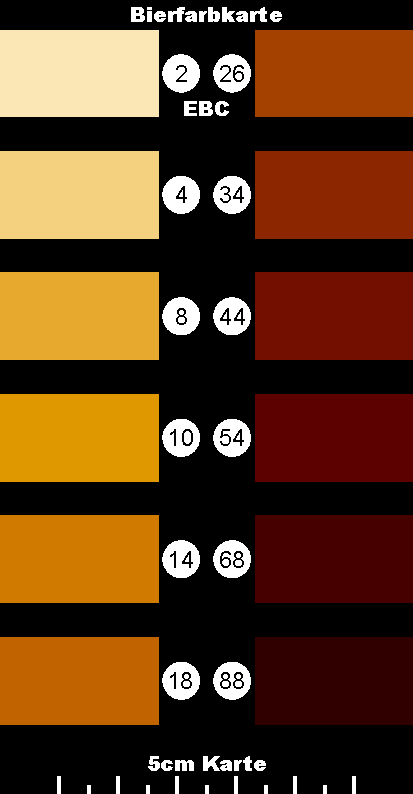
\includegraphics[width=4.8cm]{color_guide.pdf}
	\caption{Bierfarbkarte im Stil des BJCP Color Guide (Ascher, 2022)}
	\label{fig:colorguide}
\end{figure}

\section*{Bierfarbmessung}

Die \href{https://www.asbcnet.org}{ASBC} hat zwei Analysemethoden zur Messung der Bierfarbe ratifiziert: die spektralphotometrische Methode, bei der die Lichtabsorption durch eine entgaste und gefilterte Bierprobe in einer Küvette mit einer Schichtdicke von 1~cm bei einer Wellenlänge von 430~nm gemessen wird und die Tristimulus-Methode, die das Lichtspektrum in Bereich von 380--780~nm (5~nm Abstand) mit einem Kolorimeter oder einem Spektralfotometer erfasst. \parencite{ASBC2011}

Bei der spektralphotometrischen Methode erfolgt eine Messung auf Basis des bouguer-lambert-beerschen Gesetzes. Dabei wird der Transmissionsgrad ($T$) des Lichts durch eine Probe bestimmt, aus dem sich die Absorption ($A$) berechnen lässt. Der Transmissionsgrad ist der Quotient zwischen den Lichtsintensitäten nach dem Austritt ($I$) aus einer Probe und vor dem Eintritt ($I_0$) in eine Probe. Die Absorption verhält sich entlang eines gewählten Messpfads proportional. Eine Skalierung ist daher möglich, was eine Umrechnung zwischen verschiedenen Behältnisgrößen erlaubt. Es gelten folgende Zusammenhänge \parencite{deLange2016}:

\begin{equation*}
	\begin{gathered}
		T =  I / I_0 \\
		A = \log T \\		
		\textrm{EBC} = 25 \cdot A_{430}
	\end{gathered}
\end{equation*}

\begin{figure}[H]
	\centering
	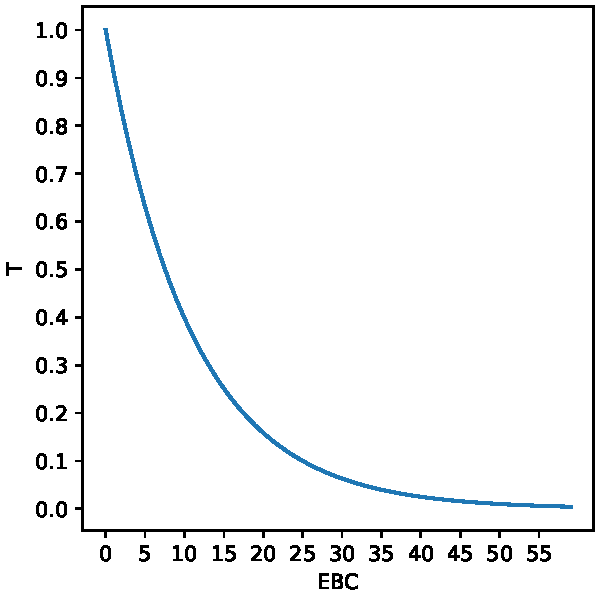
\includegraphics[width=6cm]{transmission.pdf}
	\caption{Transmissionsgrad über die EBC Skala (Ascher, 2024)}
	\label{fig:transmission}
\end{figure}


Die EBC Skala kann die Bierfarbe an sich nicht ausreichend charakterisieren, da das zugrundeliegende Verfahren nur eine Wellenlänge im blauen Bereich des sichtbaren Spektrums misst. Je nach verwendeter Schüttung kann die Bierfarbe bei gleicher Absorption visuell entweder rötlicher oder bräunlicher wahrgenommen werden \parencite{Tucker2017}. Messungen nach der Tristimulus-Methode sind nicht von der selben Problematik betroffen. Bei dieser wird das gesamte sichtbare Transmissionsspektrum gemäß dem Verfahren ASTM~E-308 zunächst in das CIE-Normvalenzsystem (XYZ-Farbraum) überführt und daraus dann anschließend ein eindeutiger Farbwert im CIELAB-Farbraum bestimmt \parencites{deLange2016}{ASBC2011}. Transformationen zu anderen Farbräumen sind ebenfalls möglich. Die entsprechenden Berechnungsvorschriften für den sRGB-Farbraum sind im Standard IEC~61966-2-1 festgelegt \parencite{W3C2015}.

\section*{Berechnung mit dem deLange Modell}

Das Modell von \cite{deLange2016} berechnet nicht direkt ein RGB-Zahlentripel im sRGB-Farbraum, sondern bildet stattdessen ein konstantes normalisiertes Bierabsorptionsspektrum ab. Unter Angabe einer spezifischen Wellenlänge $\lambda$ des Lichtspektrums in Nanometern, einer Pfadlänge $l$ in Zentimetern und dem gewünschten EBC Wert lässt sich damit ein entsprechender Transmissionsgrad $T$ bestimmen:

\begin{equation*}
T(\lambda)=\log^{-1}\left(-l \frac{\text{EBC}}{25} \left(0,02465e^{-\frac{\lambda-430}{17,591}}+0,97535e^{-\frac{\lambda-430}{82,122}}\right)\right)
\end{equation*}

Die Pfadlänge $l$ beschreibt zum Beispiel den Durchmesser eines Verkostungsglases, für das eine Farbsimulation erfolgen soll. In Verbindung mit dem BJCP Color Guide wird ein Verkostungsglas mit einem Durchmesser von 5~cm eingesetzt \parencite{BJCP}. Die \autoref{fig:ebcscale} zeigt, wie sich die Farbe bei zunehmender Pfadlänge über die EBC Skala verändert.

\begin{figure}[H]
	\centering
	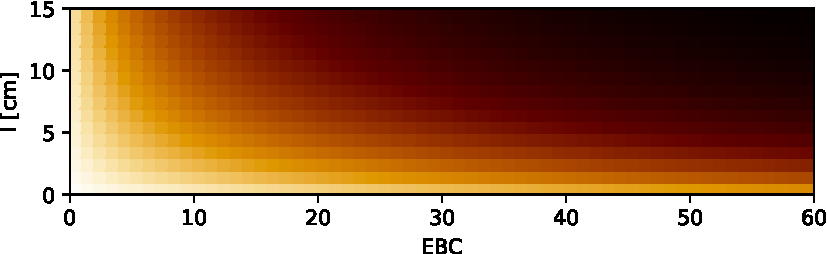
\includegraphics[width=9cm]{ebc_scale.pdf}
	\caption{Farbänderung bei zunehmender Pfadlänge (Ascher, 2024)}
	\label{fig:ebcscale}
\end{figure}

\subsection*{Transformation in den XYZ-Farbraum}

Die wahrgenommene Farbe eines Objekts ist unter anderem abhängig von der Zusammensetzung des Umgebungslichts, dem Betrachtungswinkel und der spektralen Interpretation einer Betrachterin oder eines Betrachters. Ebenfalls spielt es eine Rolle, inwieweit ein Objekt Licht reflektiert, hindurch lässt (Transmission) und welche Strahlungsleistung es hat. Das CIE-Normvalenzsystem beinhaltet kolorimetrische Verfahren, um ein Lichtspektrum unter diesen Aspekten mathematisch zu bewerten. \parencite{ASTM2022}

Mit den folgenden Formeln aus \cite{ASTM2022} und \cite{ASBC2011} lässt sich eine mit dem deLange Modell für einen bestimmten EBC Wert berechnete Spektralverteilung in den XYZ-Farbraum überführen. Bei der Summenbildung ist für $\lambda$ ein Intervall von 5~nm einzuhalten.

\begin{equation*}
	\begin{gathered}
		X = k \sum_{\lambda=380}^{780} T(\lambda) S(\lambda) \bar{x}(\lambda) \\
		Y = k \sum_{\lambda=380}^{780} T(\lambda) S(\lambda) \bar{y}(\lambda) \\
		Z = k \sum_{\lambda=380}^{780} T(\lambda) S(\lambda) \bar{z}(\lambda)
	\end{gathered}
\end{equation*}

\begin{equation*}
	k = \frac{1}{\sum_{\lambda=380}^{780} S(\lambda) \bar{y}(\lambda)}
\end{equation*}

Bei $S$ handelt es sich um eine CIE-Normbeleuchtung. Für den sRGB-Farbraum ist die tabellierte Form der D65 Normbeleuchtung anzuwenden \parencites{W3C2015}{CIE2022}. Diese entspricht Tageslicht mit einer korrelierten Farbtemperatur von 6504~K \parencite{ASTM2022}. Die tabellierten Spektralwertfunktionen des CIE-Normalbeobachters von 1931 \parencite{CIE2018} werden durch $\bar{x}$, $\bar{y}$ und $\bar{z}$ repräsentiert. Für den sRGB-Farbraum ist eine Normierung der Koordinaten im Farbraum mit der Konstante $k$ auf 1 anstatt von 100 durchzuführen \parencite{W3C2015}.

\subsection*{Transformation in den sRGB-Farbraum}

Eine Zusammenfassung der Berechnungsvorschriften des sRGB-Standards, um ein Wertetripel aus dem XYZ-Farbraum in den sRGB-Farbraum zu transformieren, ist bei \cite{W3C2015} beschrieben. Zunächst wird per Matrixmultiplikation eine Transformation zu linearen sRGB-Werten durchgeführt. Diese werden anschließend mit der $\operatorname{clip}$ Funktion auf einen Bereich von 0 bis 1 beschnitten. Werte außerhalb dieses Bereichs sind nicht mehr innerhalb des sRGB-Farbraums farbtreu darstellbar. Danach erfolgt eine Transformation zu nicht linearen sRGB-Werten mithilfe der Color Component Transfer Funktion $\operatorname{cct}$. Zur Verwendung mit Bildbearbeitungsprogramm ist es notwendig, das berechnete Ergebnis mit der Funktion $\operatorname{quant}$ auf 8-Bit zu quantifizieren. In einem Bildbearbeitungsprogramm ist der Arbeitsfarbraum vor der Übertragung des Ergebnisses auf sRGB einzustellen.

\begin{equation*}
\begin{bmatrix}
R_{l} \\
G_{l} \\
B_{l} \\
\end{bmatrix} =
\begin{bmatrix}
3,2406255 & -1,537208 & -0,4986286 \\
-0,9689307 & 1,8757561 & 0,0415175 \\
-0,0557101 & -0,2040211 & 1,0569959 \\
\end{bmatrix}
\begin{bmatrix}
X \\
Y \\
Z \\
\end{bmatrix}
\end{equation*}

\begin{equation*}
\operatorname{clip}(x)=\operatorname{max}(0, \operatorname{min}(x, 1))
\end{equation*}

\begin{equation*}
\operatorname{cct}(x)=
\begin{cases}
12,92 \cdot x & \text{für } x \leq 0,0031308, \\
1,055 \cdot x^{1/2,4} - 0,055 & \text{für } x > 0,0031308. \\
\end{cases}
\end{equation*}

\begin{equation*}
\begin{gathered}
R = \operatorname{cct}(\operatorname{clip}(R_{l})) \\
G = \operatorname{cct}(\operatorname{clip}(G_{l})) \\
B = \operatorname{cct}(\operatorname{clip}(B_{l}))
\end{gathered}
\end{equation*}

\begin{equation*}
\operatorname{quant}(x) = \lfloor (2^8-1) \cdot x \rceil
\end{equation*}

\begin{equation*}
\begin{gathered}
R_{8bit} = \operatorname{quant}(R) \\
G_{8bit} = \operatorname{quant}(G) \\
B_{8bit} = \operatorname{quant}(B)
\end{gathered}
\end{equation*}

\subsection*{Beispielimplementierung}

Im Gegensatz zu vielen Berechnungen im Heimbraubereich ist der zuvor beschriebene Algorithmus aufgrund der Anzahl der durchzuführenden Rechenschritte eher komplex. Der Autor hat deshalb dazu entschieden, eine Beispielimplementierung für mehrere Programmiersprachen im GitHub Repository \url{https://github.com/aschet/olfarve} zu hinterlegen, anstatt die Verwendung der Formeln mit einem Rechenbeispiel zu demonstrieren. Das Repository enthält auch eine Microsoft Excel im XLSX-Format (\autoref{fig:olfarve}).

\begin{figure}[H]
	\centering
	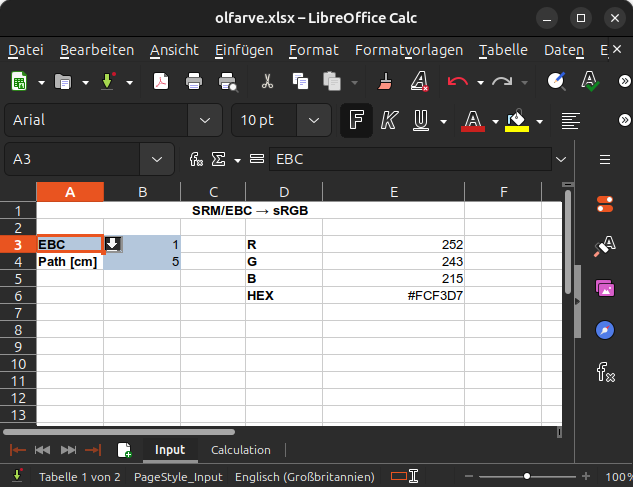
\includegraphics[width=6cm]{olfarve.png}
	\caption{XLSX Beispielimplementierung (Ascher, 2024)}
	\label{fig:olfarve}
\end{figure}

\section*{Zusammenfassung}

Mit dem deLange Modell und in den Standards ASTM~E308 und IEC~61966-2-1 beschriebenen Verfahren kann für einen EBC Wert eine Farbe im sRGB-Farbraum für verschiedene Behältnisdurchmesser simuliert werden. Hierbei ist zu beachten, dass Biere je nach eingesetzter Schüttung bei gleichen EBC Einheiten unterschiedliche Farben haben können. Das ist eine Einschränkung des zugrundeliegenden Messprinzips. Das deLange Modell kann diesen Effekt weder berücksichtigen noch kompensieren.

\printbibliography[title=Quellen]

\end{document}

